\documentclass{article}\usepackage[]{graphicx}\usepackage[]{color}
%% maxwidth is the original width if it is less than linewidth
%% otherwise use linewidth (to make sure the graphics do not exceed the margin)
\makeatletter
\def\maxwidth{ %
  \ifdim\Gin@nat@width>\linewidth
    \linewidth
  \else
    \Gin@nat@width
  \fi
}
\makeatother

\definecolor{fgcolor}{rgb}{0.345, 0.345, 0.345}
\newcommand{\hlnum}[1]{\textcolor[rgb]{0.686,0.059,0.569}{#1}}%
\newcommand{\hlstr}[1]{\textcolor[rgb]{0.192,0.494,0.8}{#1}}%
\newcommand{\hlcom}[1]{\textcolor[rgb]{0.678,0.584,0.686}{\textit{#1}}}%
\newcommand{\hlopt}[1]{\textcolor[rgb]{0,0,0}{#1}}%
\newcommand{\hlstd}[1]{\textcolor[rgb]{0.345,0.345,0.345}{#1}}%
\newcommand{\hlkwa}[1]{\textcolor[rgb]{0.161,0.373,0.58}{\textbf{#1}}}%
\newcommand{\hlkwb}[1]{\textcolor[rgb]{0.69,0.353,0.396}{#1}}%
\newcommand{\hlkwc}[1]{\textcolor[rgb]{0.333,0.667,0.333}{#1}}%
\newcommand{\hlkwd}[1]{\textcolor[rgb]{0.737,0.353,0.396}{\textbf{#1}}}%

\usepackage{framed}
\makeatletter
\newenvironment{kframe}{%
 \def\at@end@of@kframe{}%
 \ifinner\ifhmode%
  \def\at@end@of@kframe{\end{minipage}}%
  \begin{minipage}{\columnwidth}%
 \fi\fi%
 \def\FrameCommand##1{\hskip\@totalleftmargin \hskip-\fboxsep
 \colorbox{shadecolor}{##1}\hskip-\fboxsep
     % There is no \\@totalrightmargin, so:
     \hskip-\linewidth \hskip-\@totalleftmargin \hskip\columnwidth}%
 \MakeFramed {\advance\hsize-\width
   \@totalleftmargin\z@ \linewidth\hsize
   \@setminipage}}%
 {\par\unskip\endMakeFramed%
 \at@end@of@kframe}
\makeatother

\definecolor{shadecolor}{rgb}{.97, .97, .97}
\definecolor{messagecolor}{rgb}{0, 0, 0}
\definecolor{warningcolor}{rgb}{1, 0, 1}
\definecolor{errorcolor}{rgb}{1, 0, 0}
\newenvironment{knitrout}{}{} % an empty environment to be redefined in TeX

\usepackage{alltt}
\setlength\parindent{0pt}
\IfFileExists{upquote.sty}{\usepackage{upquote}}{}

\begin{document}



\begin{knitrout}
\definecolor{shadecolor}{rgb}{0.969, 0.969, 0.969}\color{fgcolor}\begin{kframe}
\begin{alltt}
\hlstd{dat}\hlkwb{<-}\hlkwd{read.table}\hlstd{(}\hlkwc{file}\hlstd{=}\hlstr{"pop.csv"}\hlstd{,}\hlkwc{header}\hlstd{=T)}
\hlkwd{head}\hlstd{(dat,}\hlnum{5}\hlstd{)}
\end{alltt}
\begin{verbatim}
##   t ID     z     bvs    C s ARS age p1 p2 phi
## 1 1  2 11.61  0.8402  249 M   0   1 NA NA   1
## 2 1  3 13.14  1.0114  587 F  26   1 NA NA   1
## 3 1  4 13.71  0.2694 2427 M   0   1 NA NA   1
## 4 1  5 10.88 -0.9088   89 F   5   1 NA NA   1
## 5 1  8 10.94  0.2045   85 F   7   1 NA NA   1
\end{verbatim}
\begin{alltt}
\hlkwd{which}\hlstd{(}\hlopt{!}\hlstd{(}\hlkwd{min}\hlstd{(dat}\hlopt{$}\hlstd{ID)}\hlopt{:}\hlkwd{max}\hlstd{(dat}\hlopt{$}\hlstd{ID)}\hlopt\hlstd{dat}\hlopt{$}\hlstd{ID))}
\end{alltt}
\begin{verbatim}
## integer(0)
\end{verbatim}
\end{kframe}
\end{knitrout}


\begin{knitrout}
\definecolor{shadecolor}{rgb}{0.969, 0.969, 0.969}\color{fgcolor}\begin{kframe}
\begin{alltt}
\hlstd{dat2}\hlkwb{<-}\hlkwd{subset}\hlstd{(dat,phi}\hlopt{==}\hlnum{1}\hlstd{)}
\hlstd{dat2}\hlkwb{<-}\hlstd{dat2[,}\hlkwd{c}\hlstd{(}\hlstr{"ID"}\hlstd{,}\hlstr{"t"}\hlstd{,}\hlstr{"z"}\hlstd{)]}
\hlkwd{library}\hlstd{(}\hlstr{'reshape'}\hlstd{)}
\end{alltt}


{\ttfamily\noindent\itshape\color{messagecolor}{\#\# Loading required package: plyr\\\#\# \\\#\# Attaching package: 'reshape'\\\#\# \\\#\# The following objects are masked from 'package:plyr':\\\#\# \\\#\#\ \ \ \  rename, round\_any}}\begin{alltt}
\hlkwd{par}\hlstd{(}\hlkwc{mar}\hlstd{=}\hlkwd{c}\hlstd{(}\hlnum{6}\hlstd{,}\hlnum{6}\hlstd{,}\hlnum{2}\hlstd{,}\hlnum{2}\hlstd{))}
\hlstd{dat3}\hlkwb{<-}\hlkwd{reshape}\hlstd{(dat2,} \hlkwc{idvar} \hlstd{=} \hlstr{"ID"}\hlstd{,} \hlkwc{timevar} \hlstd{=} \hlstr{"t"}\hlstd{,} \hlkwc{direction} \hlstd{=} \hlstr{"wide"}\hlstd{)}
\hlkwa{for}\hlstd{(i} \hlkwa{in} \hlnum{2}\hlopt{:}\hlstd{(}\hlkwd{ncol}\hlstd{(dat3)}\hlopt{-}\hlnum{2}\hlstd{))\{}
  \hlkwd{plot}\hlstd{(dat3[,i],dat3[,i}\hlopt{+}\hlnum{1}\hlstd{],}\hlkwc{main}\hlstd{=}\hlkwd{paste}\hlstd{(}\hlstr{"Year"}\hlstd{,i}\hlopt{-}\hlnum{1}\hlstd{),}\hlkwc{xlab}\hlstd{=}\hlkwd{paste}\hlstd{(}\hlstr{"z("}\hlstd{,i}\hlopt{-}\hlnum{1}\hlstd{,}\hlstr{")"}\hlstd{,}\hlkwc{sep}\hlstd{=}\hlstr{""}\hlstd{),}\hlkwc{ylab}\hlstd{=}\hlkwd{paste}\hlstd{(}\hlstr{"z("}\hlstd{,i,}\hlstr{")"}\hlstd{,}\hlkwc{sep}\hlstd{=}\hlstr{""}\hlstd{))}
\hlstd{\}}
\hlstd{temp}\hlkwb{<-}\hlstd{dat[,}\hlopt{-}\hlkwd{c}\hlstd{(}\hlstr{"t"}\hlstd{,}\hlstr{"z"}\hlstd{)]}
\end{alltt}


{\ttfamily\noindent\bfseries\color{errorcolor}{\#\# Error: invalid argument to unary operator}}\begin{alltt}
\hlstd{temp}\hlkwb{<-}\hlstd{temp[}\hlopt{!}\hlkwd{duplicated}\hlstd{(temp),]}
\end{alltt}


{\ttfamily\noindent\bfseries\color{errorcolor}{\#\# Error: object 'temp' not found}}\begin{alltt}
\hlstd{dat4}\hlkwb{<-}\hlkwd{merge}\hlstd{(dat3,temp,}\hlkwc{by}\hlstd{=}\hlstr{"ID"}\hlstd{)}
\end{alltt}


{\ttfamily\noindent\bfseries\color{errorcolor}{\#\# Error: object 'temp' not found}}\begin{alltt}
\hlstd{dat4}
\end{alltt}


{\ttfamily\noindent\bfseries\color{errorcolor}{\#\# Error: object 'dat4' not found}}\end{kframe}
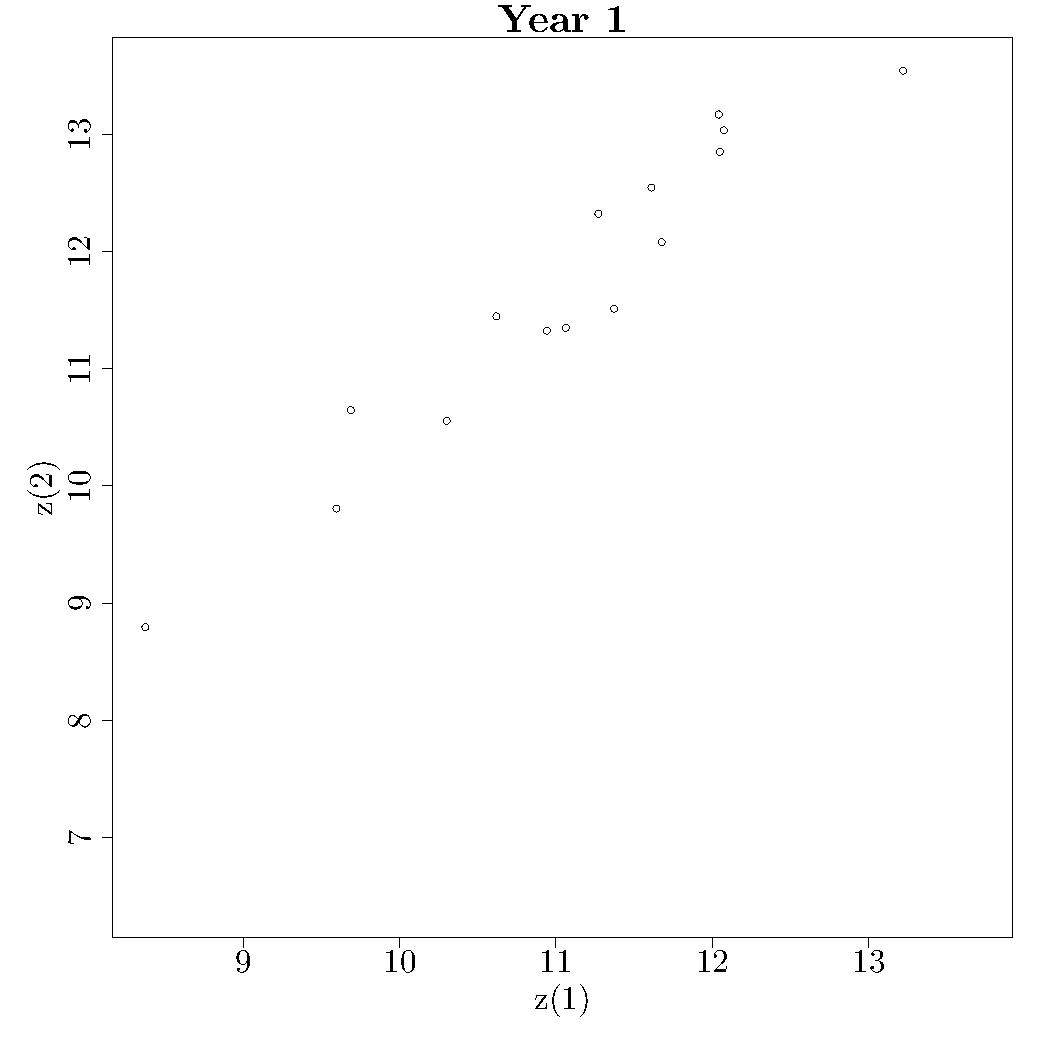
\includegraphics[width=0.35\textwidth]{figure/Reshaping1} 
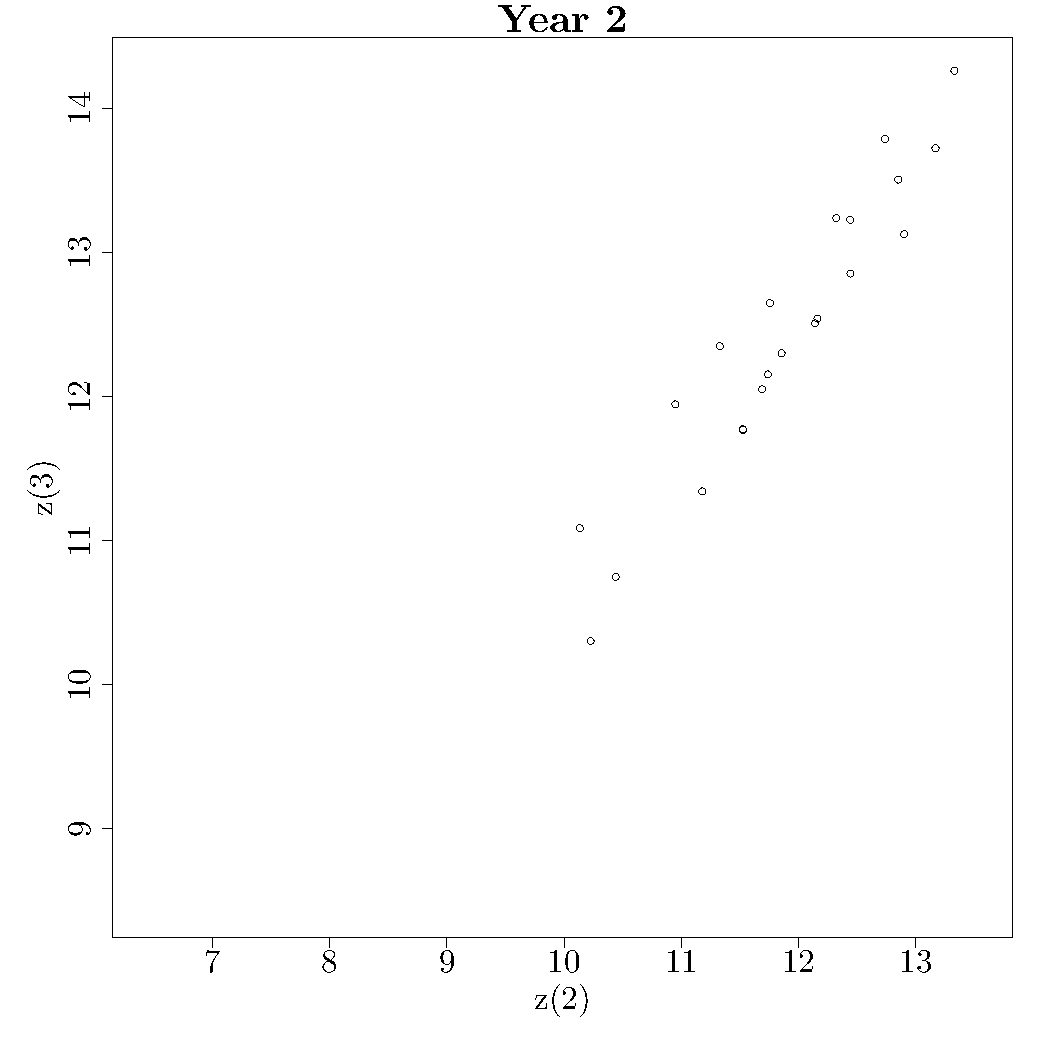
\includegraphics[width=0.35\textwidth]{figure/Reshaping2} 
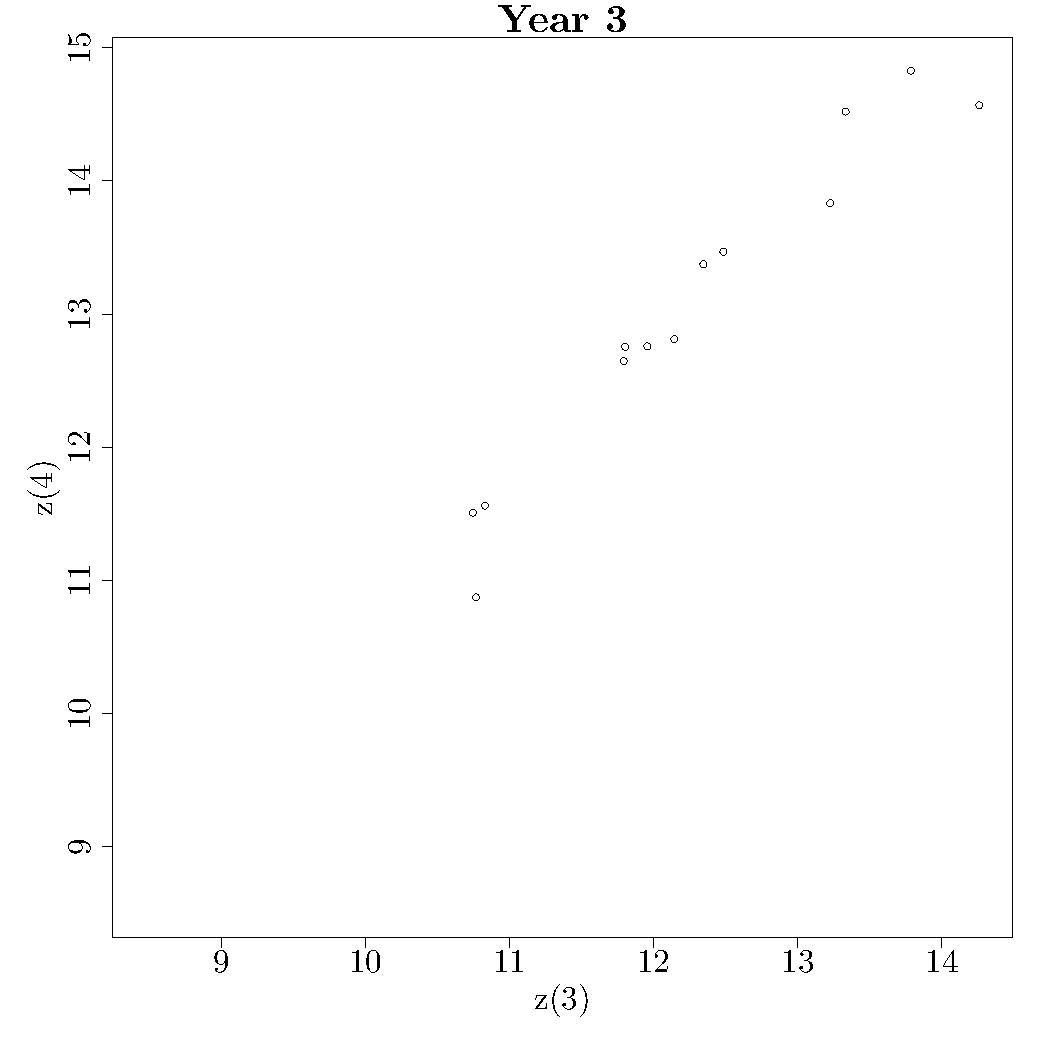
\includegraphics[width=0.35\textwidth]{figure/Reshaping3} 
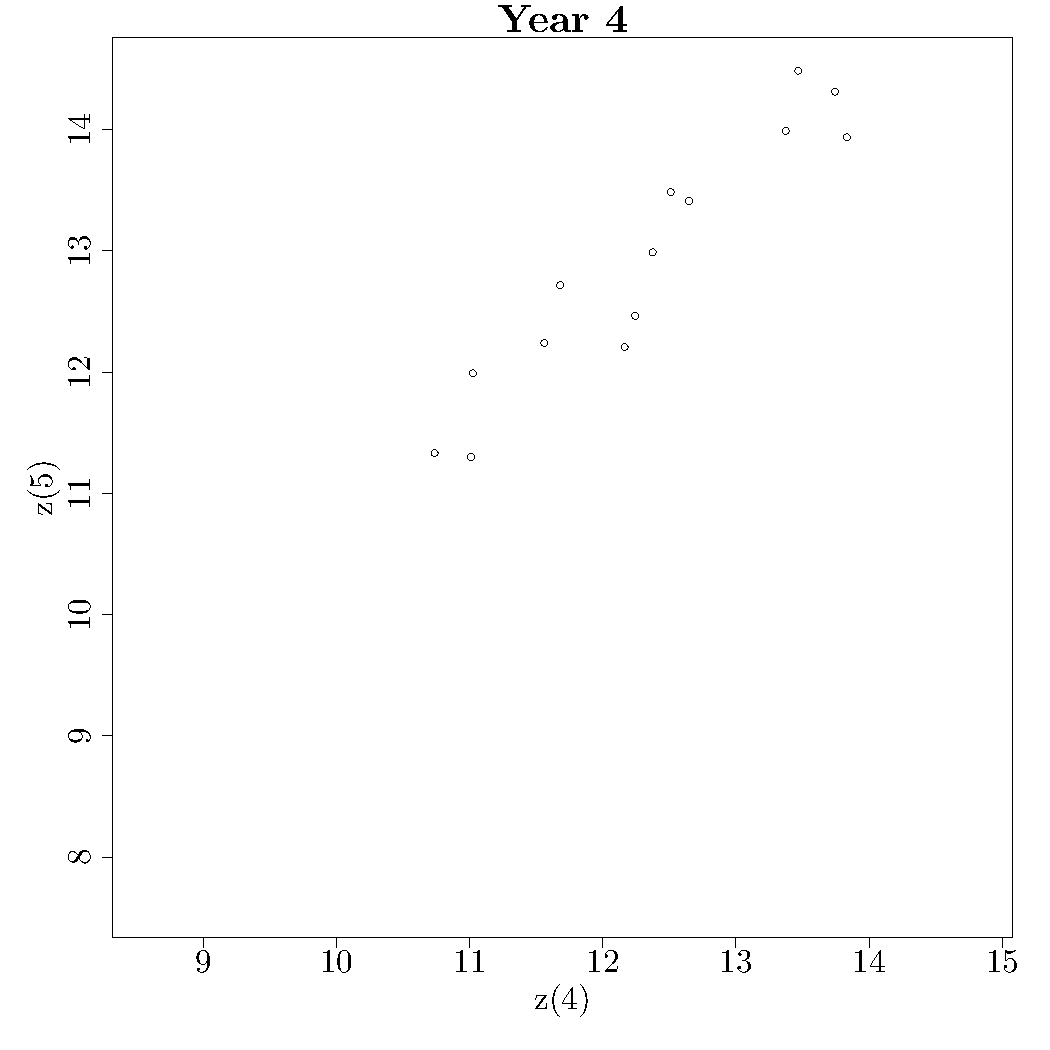
\includegraphics[width=0.35\textwidth]{figure/Reshaping4} 
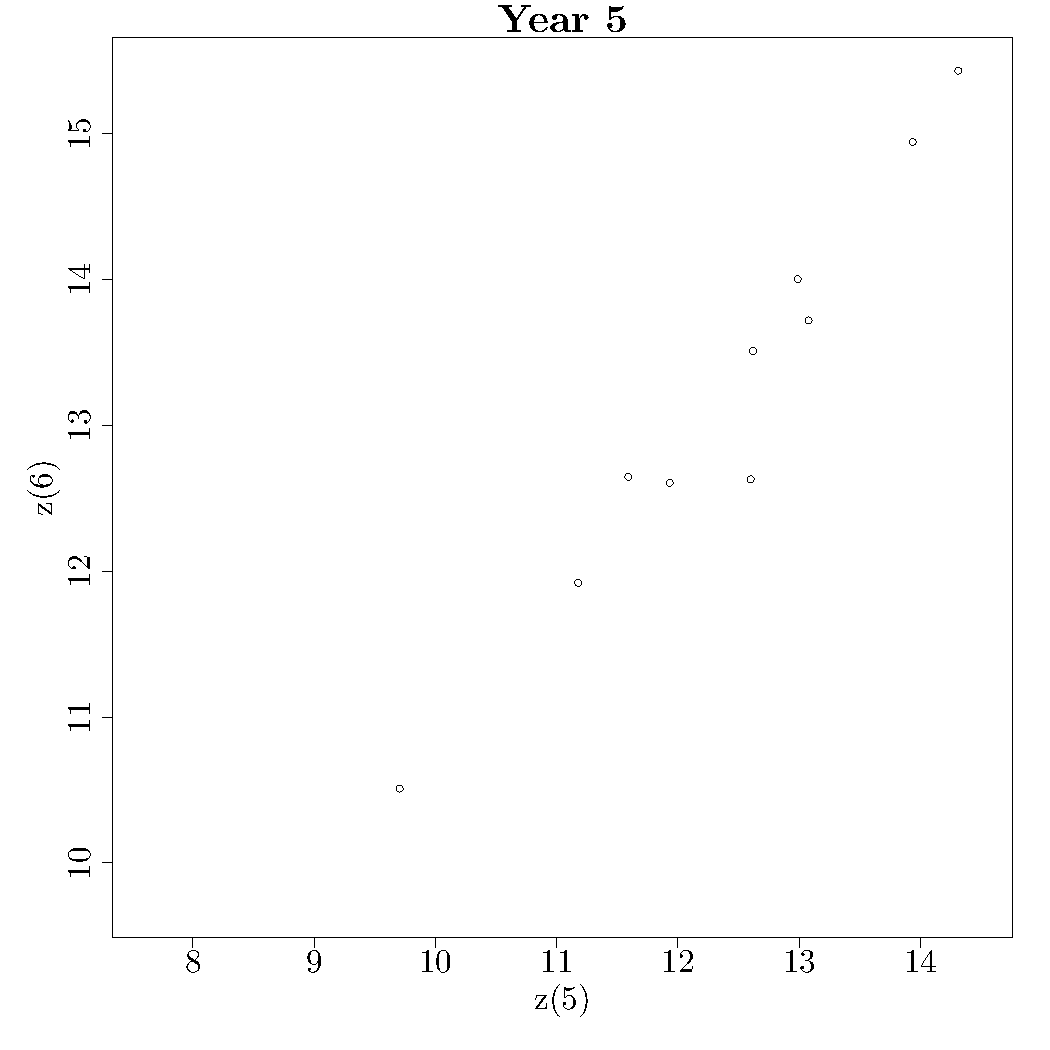
\includegraphics[width=0.35\textwidth]{figure/Reshaping5} 
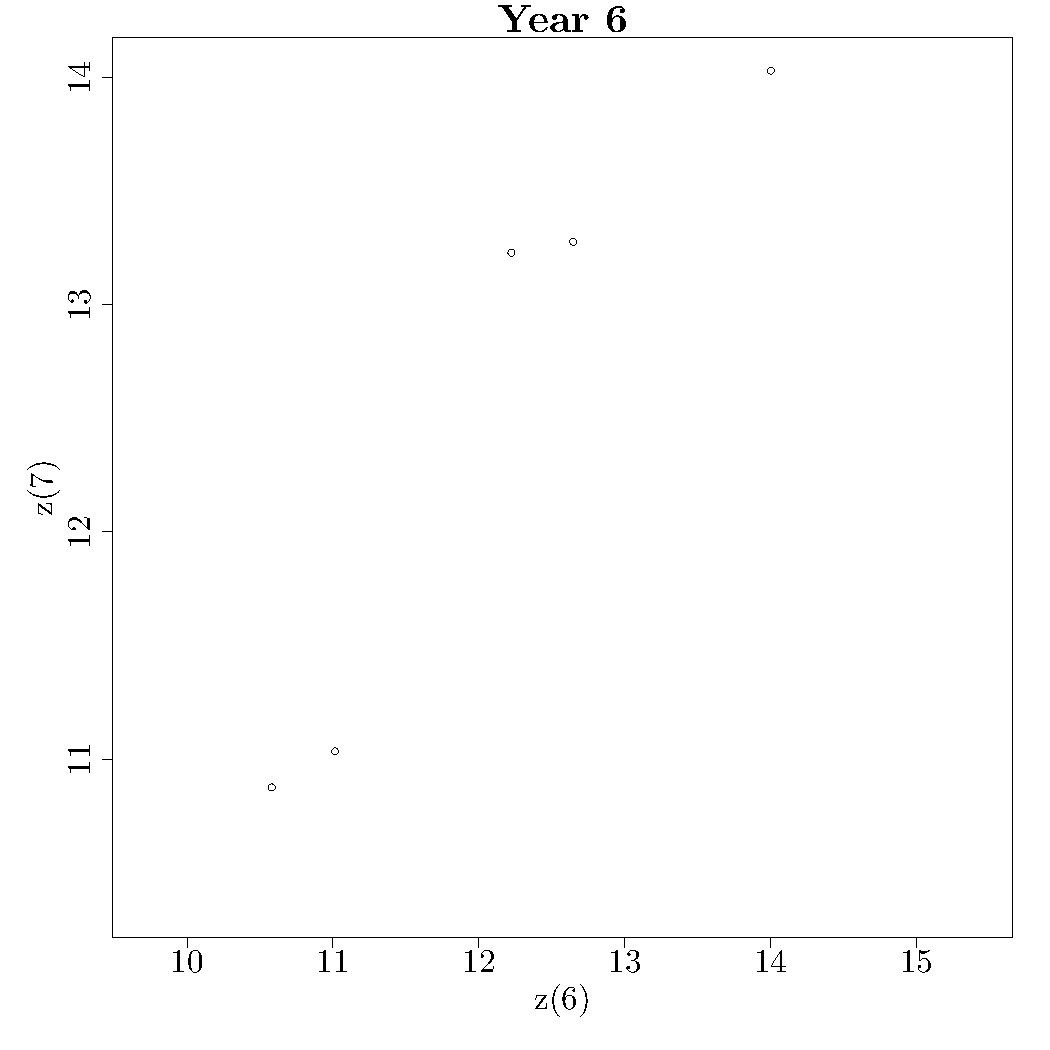
\includegraphics[width=0.35\textwidth]{figure/Reshaping6} 
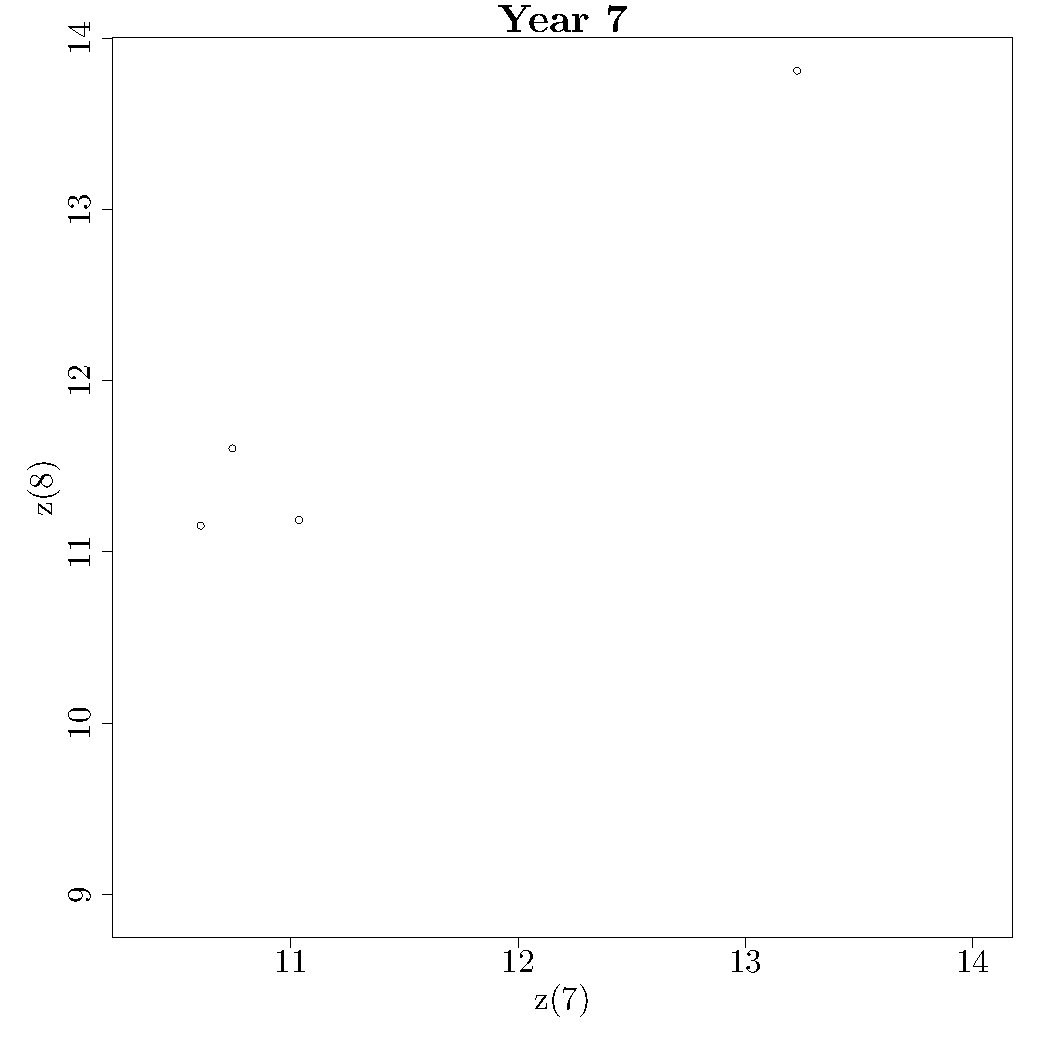
\includegraphics[width=0.35\textwidth]{figure/Reshaping7} 
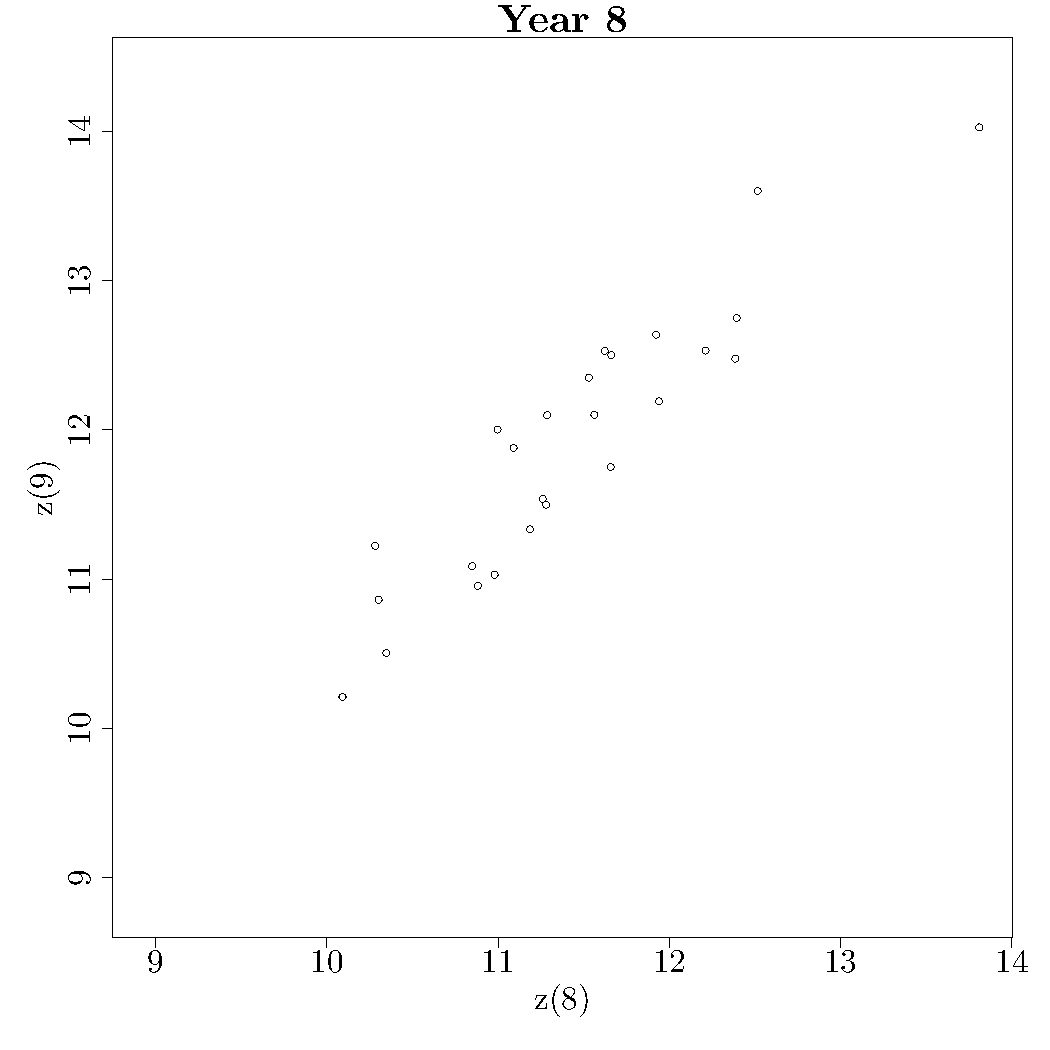
\includegraphics[width=0.35\textwidth]{figure/Reshaping8} 
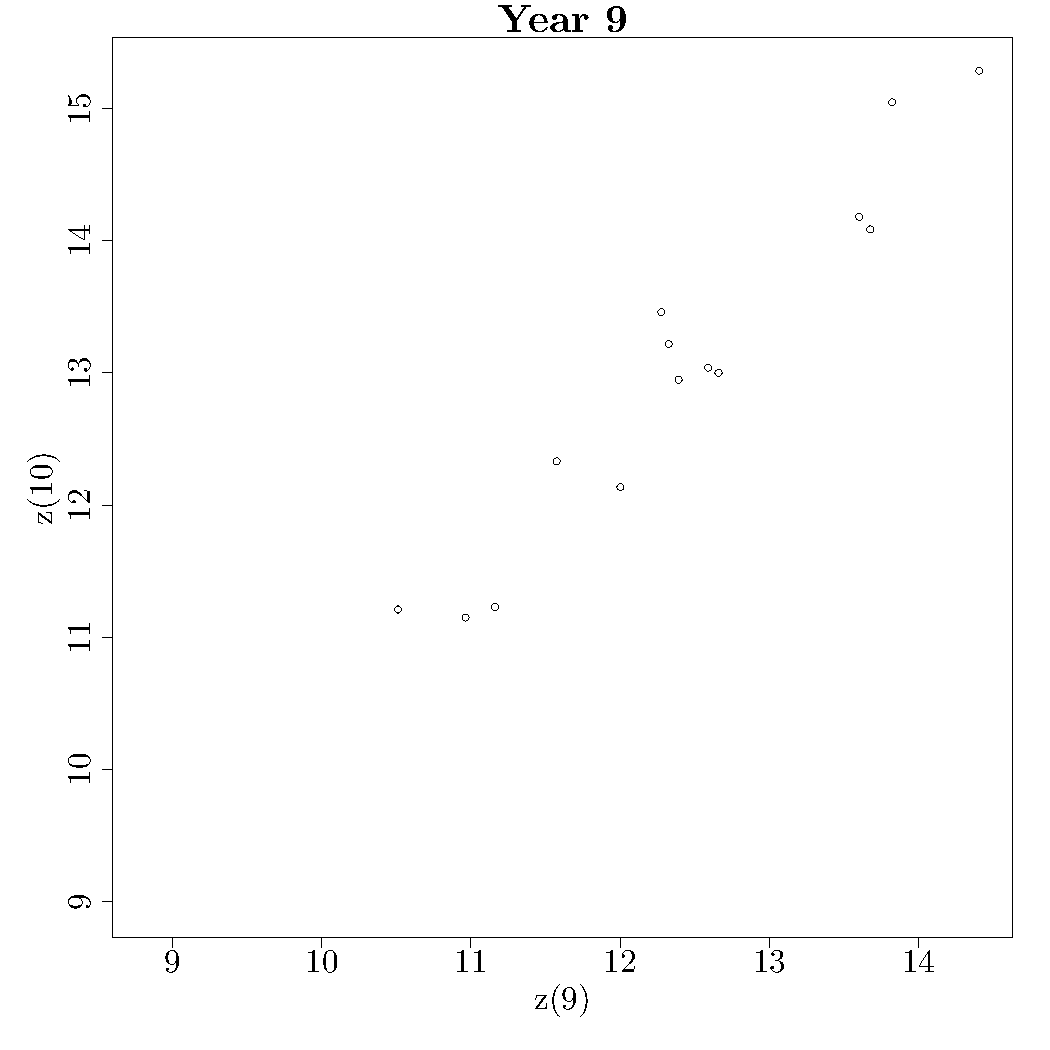
\includegraphics[width=0.35\textwidth]{figure/Reshaping9} 
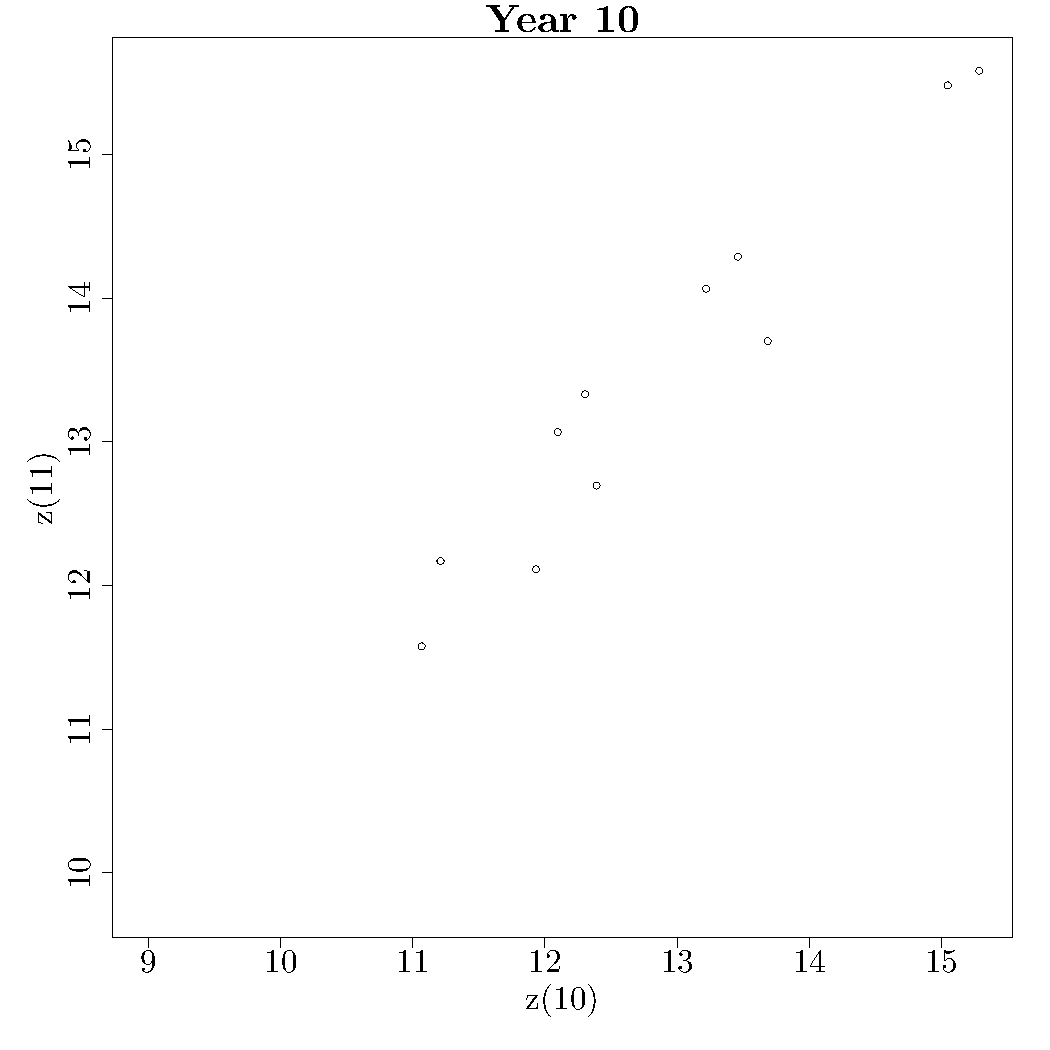
\includegraphics[width=0.35\textwidth]{figure/Reshaping10} 
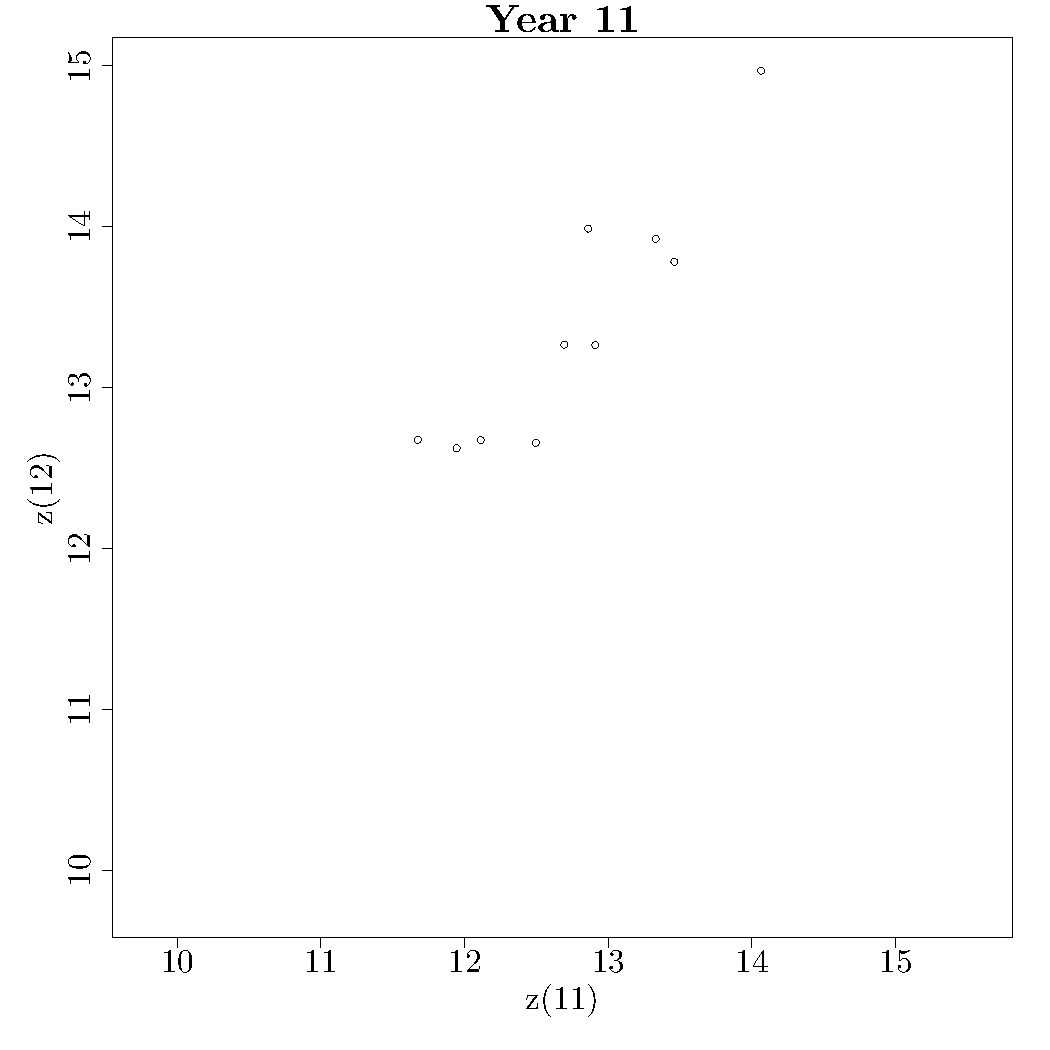
\includegraphics[width=0.35\textwidth]{figure/Reshaping11} 
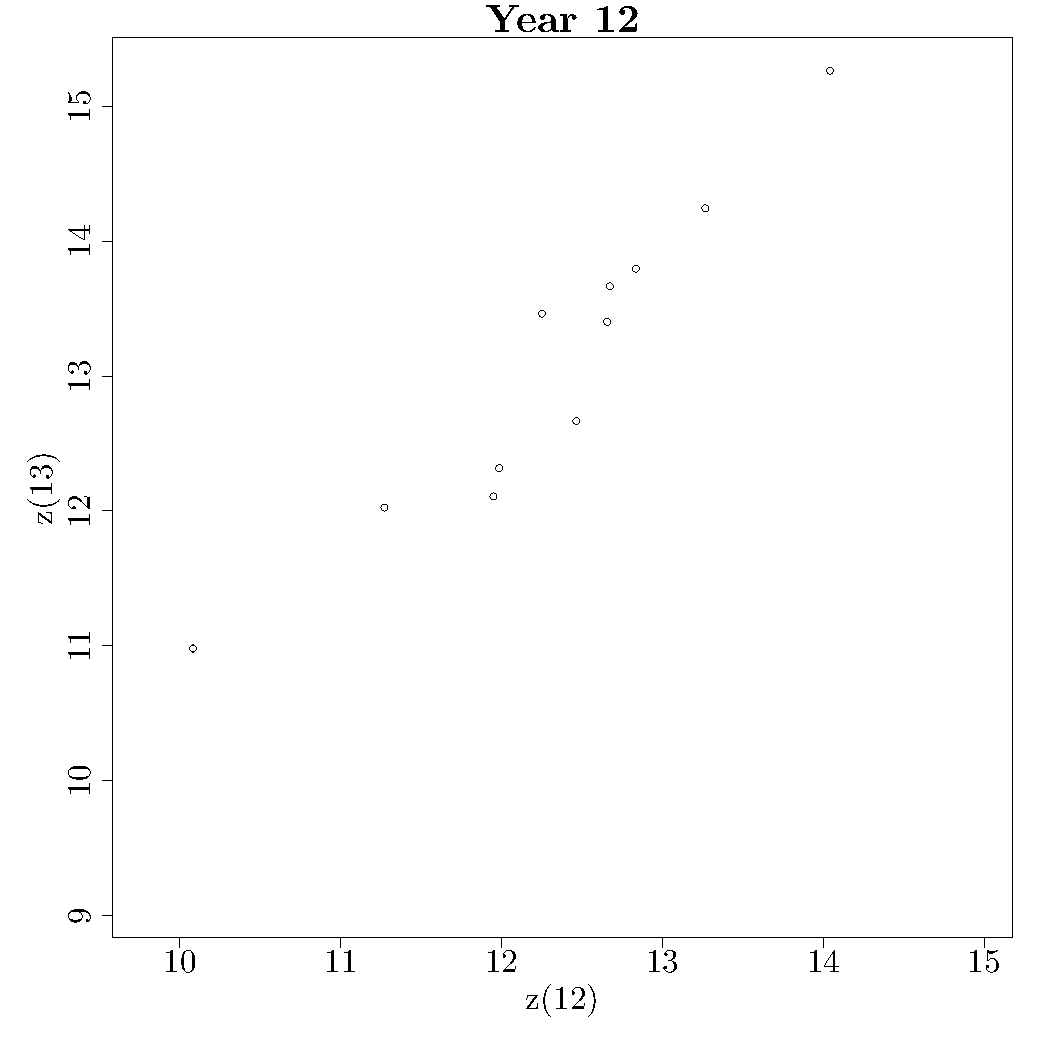
\includegraphics[width=0.35\textwidth]{figure/Reshaping12} 
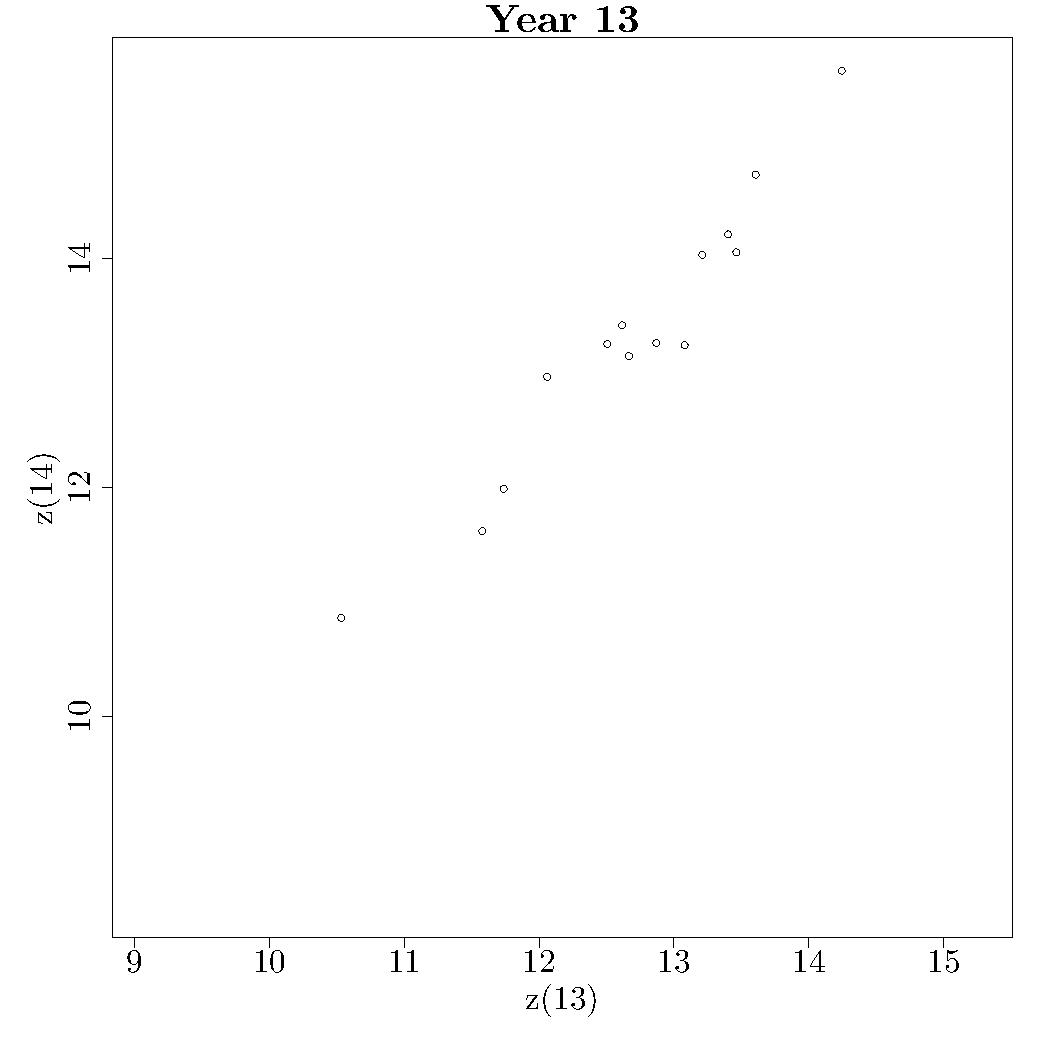
\includegraphics[width=0.35\textwidth]{figure/Reshaping13} 
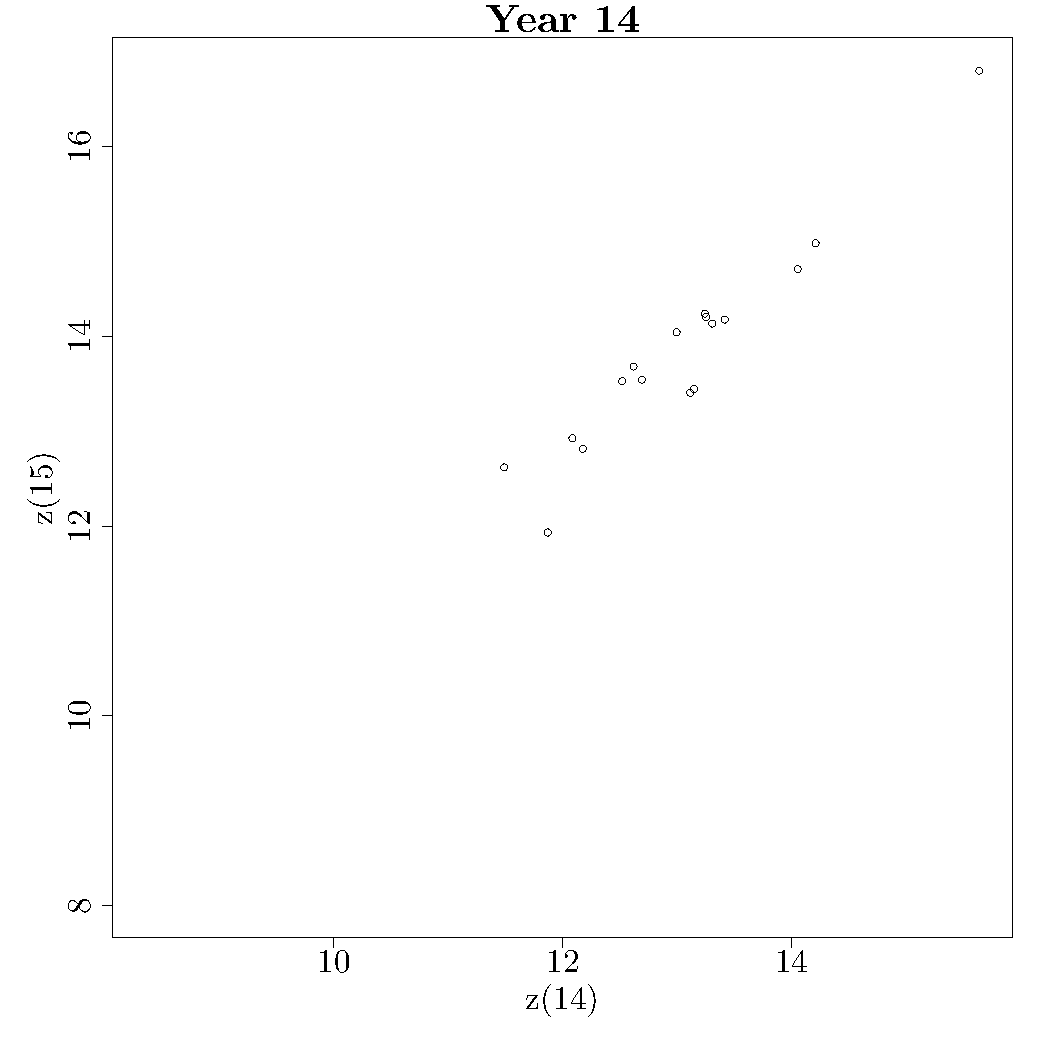
\includegraphics[width=0.35\textwidth]{figure/Reshaping14} 
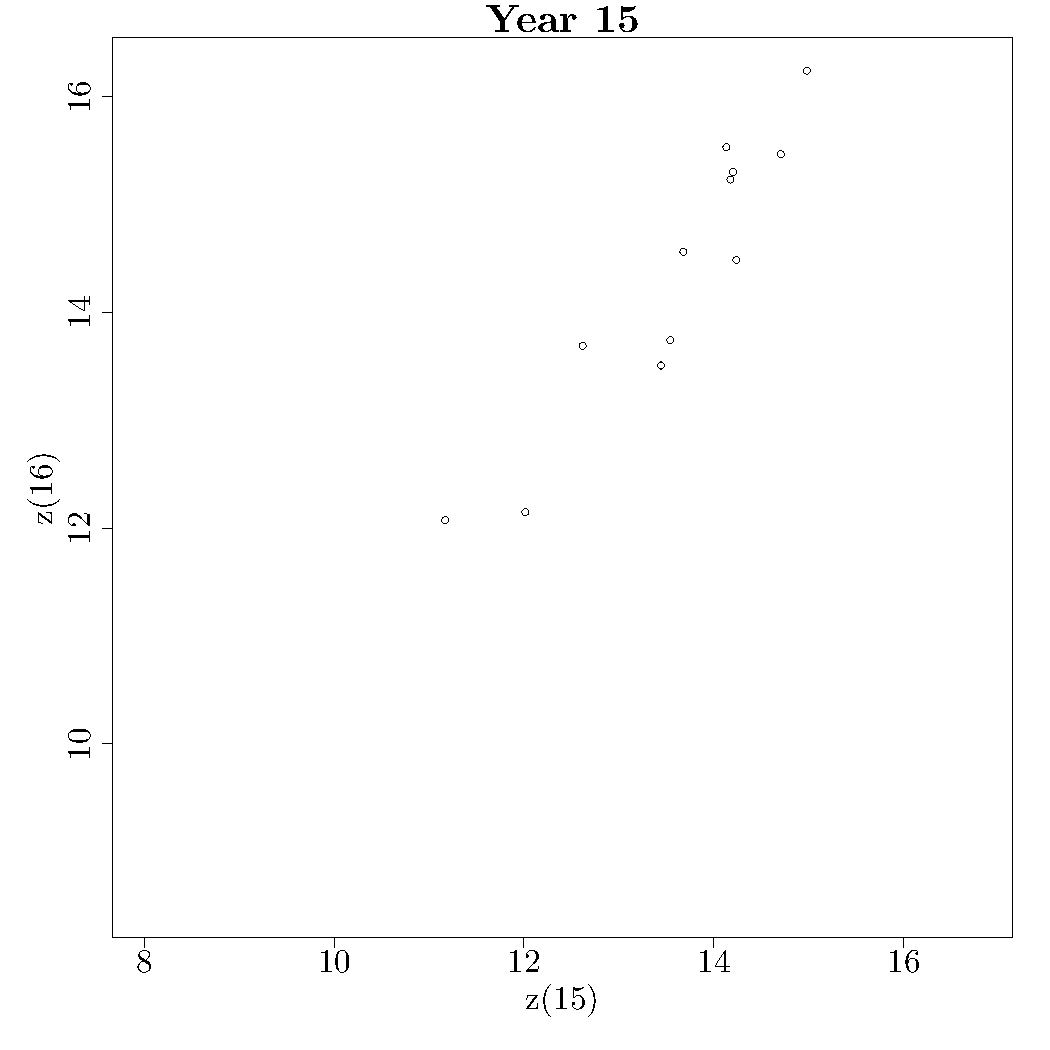
\includegraphics[width=0.35\textwidth]{figure/Reshaping15} 
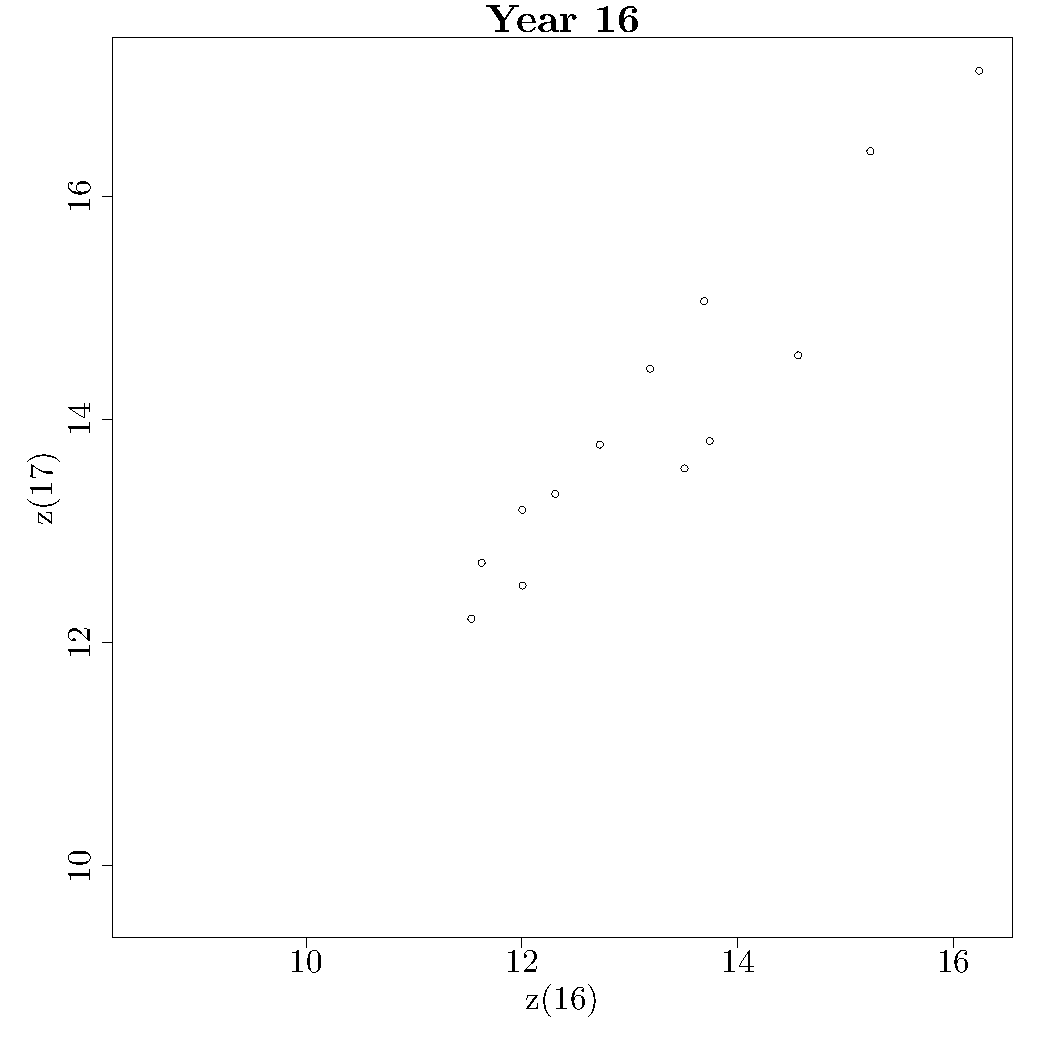
\includegraphics[width=0.35\textwidth]{figure/Reshaping16} 
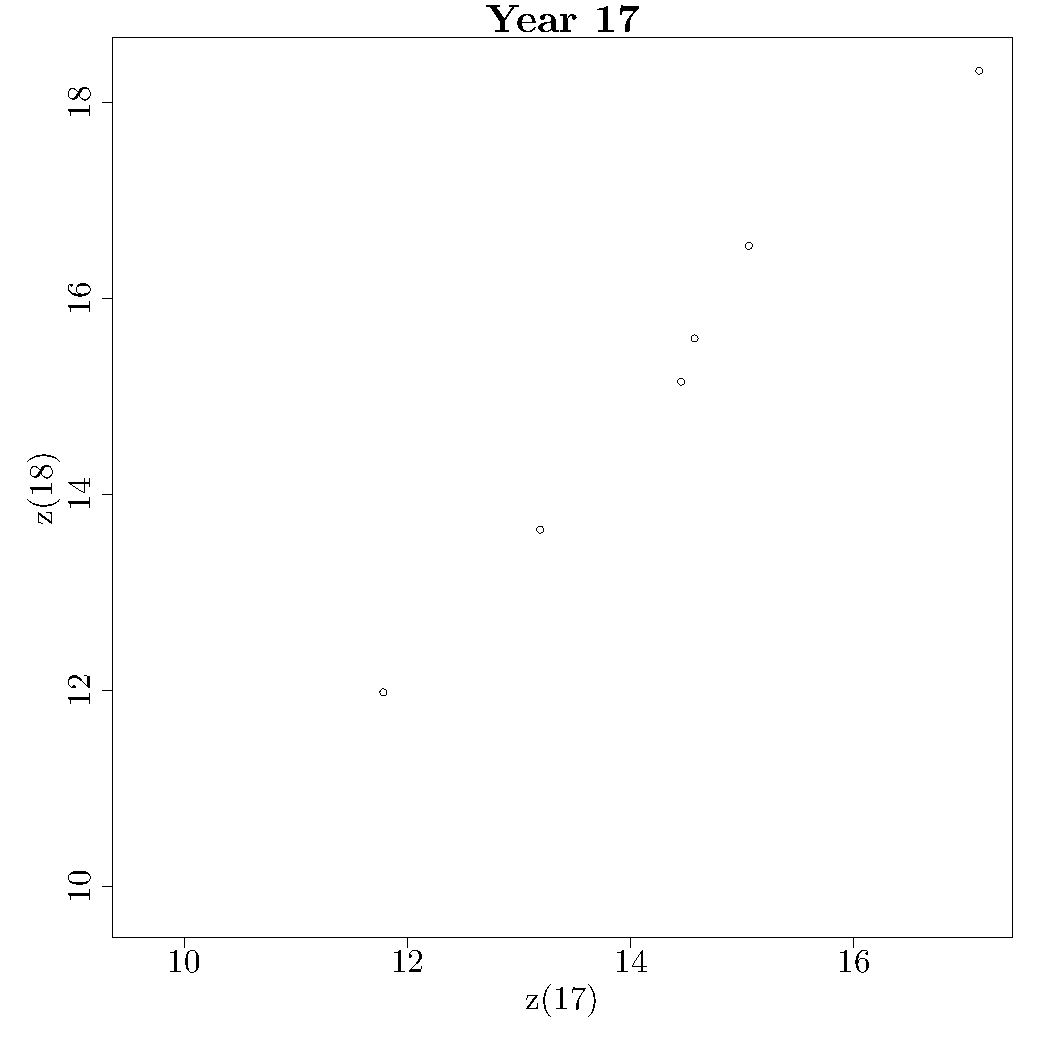
\includegraphics[width=0.35\textwidth]{figure/Reshaping17} 

\end{knitrout}



\end{document}
